\documentclass[12pt]{article}
\usepackage{amssymb, amsmath, amsfonts, bm, graphicx, geometry}
\usepackage{tabularx, booktabs, float, enumitem, multicol, mathtools}
\geometry{margin=1in}


\title{}
\date{}
\author{}

\begin{document}
\begin{center}
{\LARGE ESC-221 Basic Principles of Electrical Engineering\par}
\end{center}
The main goal of this course is to be able to model real world circuits using basic circuit elements and to be able to analyze these circuits using the fundamental laws of circuit analysis.
\section*{Systems of Units}
\textbf{SI Prefixes}
\[\begin{aligned}
\text{femto (f)}  &= 10^{-15} \\
\text{pico (p)}   &= 10^{-12} \\
\text{nano (n)}   &= 10^{-9} \\
\text{micro ($\mu$)}  &= 10^{-6} \\
\text{milli (m)}  &= 10^{-3} \\
\text{centi (c)}  &= 10^{-2} \\
\text{deci (d)}   &= 10^{-1} \\
\text{deca (da)}  &= 10^{1} \\
\text{hecto (h)}  &= 10^{2} \\
\text{kilo (k)}   &= 10^{3} \\
\text{mega (M)}   &= 10^{6} \\
\text{giga (G)}   &= 10^{9} \\
\text{tera (T)}   &= 10^{12} \\
\text{peta (P)}   &= 10^{15} \\
\end{aligned}\]
\textbf{Work and Energy}\\
Recall that work is the product of power and time, thus energy is given by $\boxed{1\,\text{J} = 1\,\text{W} \times 1\,\text{s}}$. Energy is usually measured in \textbf{watt hours (Wh)} where \boxed{1\,\text{Wh} = 3600\,\text{J}}.\\\\
\textbf{Battery capacity} (energy stored) is then also given in terms of Wh. Since the voltage of a battery is constant, we can define the energy stored in terms of the charge capacity $Q$ (in Ampere hours, Ah) and voltage $V$ (in Volts, V) as:
\[w = \int P\,dt = \int VI\,dt = V\int I\,dt = VQ\quad\text{or}\quad P\Delta t\]
where $Q$ is in [Ah], $V$ is in [V], and $w$ is in [Wh].\\\\
\underline{Note:} We can pull voltage and current out of the integral for DC circuits since they are constant with time.\\\\
To find how long the battery will last, we can divide its battery capacity by the load/output power.
\[t = \frac{w}{P}\quad \frac{\text{[Wh]}}{\text{[W]}}\]
To find how long it will take to charge the battery, we can divide its charge capacity by the charging current.
\[t = \frac{Q}{I_{\text{eff}}}\quad \left(I_{\text{eff}} = \frac{Q}{t}\right)\]
Where $I_{eff}$ is the effective charging current accounting for any losses ($I_{eff} = I_{in} \times \eta$ where $\eta$ is the efficiency of the charger).
\section*{Charge}
The charge of an electron is given in coulombs as $\boxed{1.602 \times 10^{-19}\,\text{C}}$.\\\\
Charge is conserved!
\section*{Current}
Moving charges create current. Conventional current is defined as the flow of positive charge and is in the opposite direction of actual electron flow. The unit of current is the ampere (A) where \boxed{1\,\text{A} = 1\,\text{C/s}}.
\[\boxed{i\equiv\frac{dq}{dt}}\]
\textbf{Direct Current} is denoted by $I$ and stays constant with time.\\\\
\textbf{Alternating Current} is denoted by $i(t)$ and varies sinusoidally with time.\\\\
\underline{Note:} The sign of the current indicates the direction in which the charge is moving with reference to the direction of interest defined (we just need to pick a direction and stay consistent). A negative current just means that it is flowing in the opposite direction to the one we defined as positive.
\section*{Voltage}
Current flows when there is a difference in charge between two locations. This is represented by a potential difference of voltage (V).\\\\
Voltage is equal to the energy needed to move a single charge between two locations. Moving from a higher to lower potential yields energy, while moving from a lower to higher potential requires energy. The unit of voltage is the volt (V) where \boxed{1\,\text{V} = 1\,\text{J/C}}.
\section*{Power}
Power is the rate of at which energy is transferred.
\[\boxed{P \equiv \frac{dw}{dt}}\]
Circuit elements that \textit{absorb} power have positive power.\\\\
Circuit elements that \textit{generate} power have negative power.\\\\
The power required to push a current $I$ through a voltage $V$ is given by:
\[\boxed{P = VI}\]
Power is given in watts (W) where \boxed{1\,\text{W} = 1\,\text{J/s}}.\\\\
\underline{Note:} The sign convention is consistent with the signs of the voltage and current. If current enters the positive terminal, then power is being absorbed. If current enters the negative terminal, then power is being generated.
\section*{Circuit Elements}
\textbf{Independent Sources}\\
Independent sources provides a specified voltage or current regardless of the other elements in the circuit. In an ideal independent voltage source, its voltage is constant but the current it supplies depends on the rest of the circuit. Likewise, in an ideal independent current source, its current is constant but the voltage across it depends on the rest of the circuit.
\begin{center}
    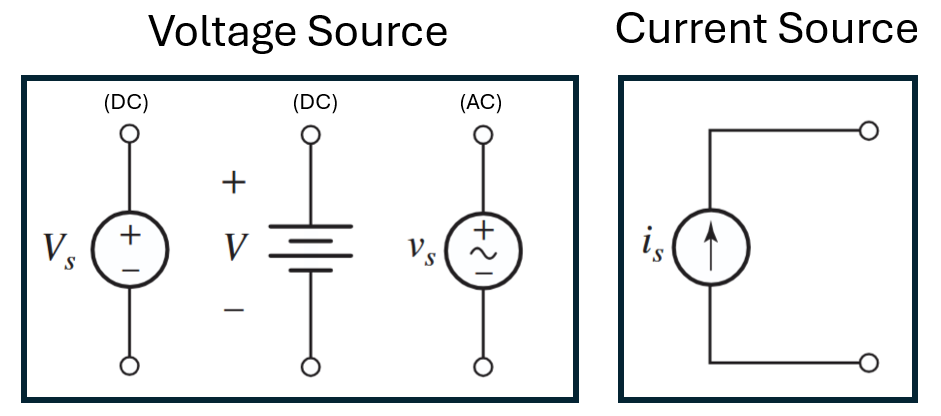
\includegraphics[width=0.5\textwidth]{Sources.png}
\end{center}
\textbf{Dependent Sources}\\
\begin{minipage}{0.5\textwidth}
For dependent sources, the voltage or current it provides depends on a function of the voltage or current elsewhere in the circuit. There are four types of dependent sources: (a) current-controlled current
source; (b) voltage-controlled current source; (c) voltage-controlled voltage source; (d) current-controlled voltage source.
\end{minipage}
\hfill
\begin{minipage}{0.45\textwidth}
    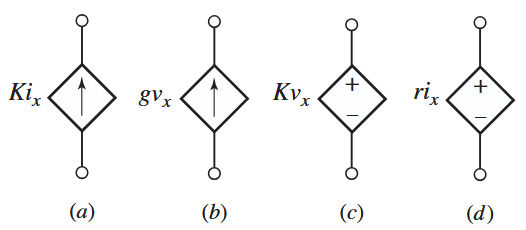
\includegraphics[width=\textwidth]{Dependent Sources.png}
\end{minipage}
\section*{Resistance}
All materials resist the flow of current. Resistance is the quantifies this in units of ohms ($\Omega$). The resistance of a cylinder of length $l$ and cross-sectional area $A$ is given by:
\[\boxed{R = \rho \frac{l}{A}}\]
where $\rho$ is the resistivity of the material.\\\\
\textbf{Conductance}\\
Conductance is the reciprocal of resistance and is measured in siemens (S).
\[\boxed{G = \frac{1}{R} = \sigma \frac{A}{l}}\]
where $\sigma$ is the conductivity of the material.
\section*{Ohm's Law}
Relationship between the voltage and current flowing through a circuit element is given by Ohm's Law:
\[\boxed{V = IR}\]
Using Ohm's Law, we can also express power as:
\[\boxed{P = VI = I^2R = \frac{V^2}{R}}\]
\section*{Open and Short Circuits}
A \textbf{short circuit} is defined as a wire with zero resistance, and thus corresponds to a voltage of 0 V across its terminals.\\\\
An \textbf{open circuit} is defined as a break in the circuit with infinite resistance, and thus corresponds to a current of 0 A through its terminals.
\section*{Nodes, Paths, Loops, Branches}
A \textbf{node} is a point in a circuit where two or more circuit elements meet.\\\\
A \textbf{branch} is a single circuit element connected between two nodes.\\\\
A \textbf{path} is a sequence of connected elements that does not pass through any node more than once.
If the path starts and ends at the same node, it is a \textbf{loop}.
\section*{Kirchoff's Voltage Law}
The sum of voltages around any closed loop in a circuit must equal zero (conservation of energy).
\section*{Kirchoff's Current Law}
The sum of currents entering any node must equal the sum of currents leaving that node or a closed boundary (conservation of charge).
\section*{Series Connections}
Elements are in series if they are connected such that the same current flows through each element.
\textbf{Resistors in Series}
\[\boxed{R_{\text{eq}} = R_1 + R_2 + \cdots + R_n}\]
\begin{center}
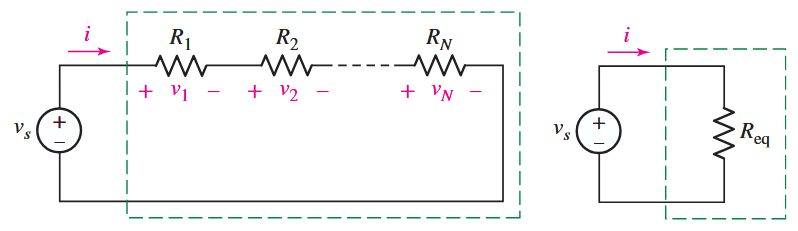
\includegraphics[width=0.6\textwidth]{Series.png}
\end{center}
\section*{Parallel Connections}
Elements are in parallel if they are connected such that the same voltage is across each element.
\textbf{Resistors in Parallel}
\[\boxed{R_{\text{eq}} = \frac{1}{\frac{1}{R_1} + \frac{1}{R_2} + \cdots + \frac{1}{R_n}}}\]
\begin{center}
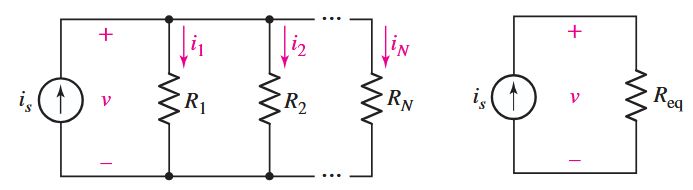
\includegraphics[width=0.6\textwidth]{Parallel.png}
\end{center}\newpage
\section*{Series and Parallel Sources}
Voltage sources in series add up algebraically
\begin{center}
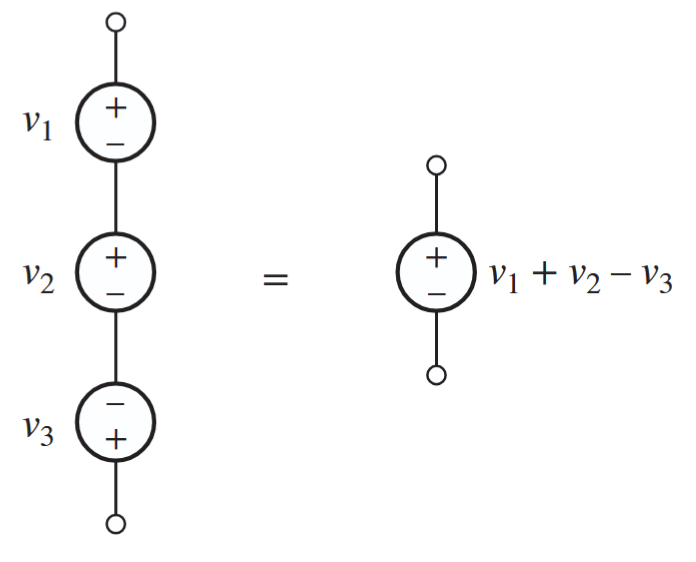
\includegraphics[width=0.5\textwidth]{Series V.png}
\end{center}
Current sources in parallel add up algebraically
\begin{center}
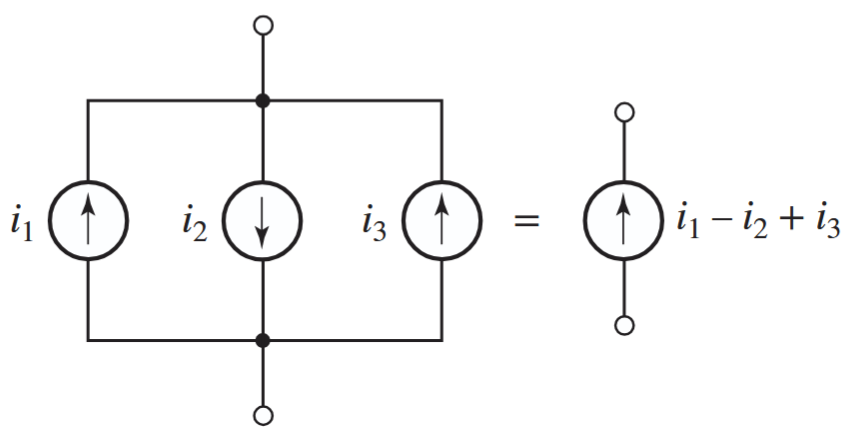
\includegraphics[width=0.5\textwidth]{Parallel C.png}
\end{center}
\section*{Nodal Analysis}
Nodal analysis is a direct application of KCL at the nodes of a circuit, to use it we follow these steps:
\begin{enumerate}
  \item Choose a reference node (ground $V=0$). Choose the node with the most connections to be the reference node.
  \item Assign node voltages (unknowns) to the remaining nodes with respect to the reference node.
  \item Apply KCL, using Ohm's law to express currents in terms of node voltages. For example if a resistor $R_1$ is between node 1 and node 2, then the current from node 1 to node 2 is given by 
  \[I_{R_1} = \frac{V_1 - V_2}{R_1}\]
  \item Solve the resulting system of equations for the unknown node voltages.
\end{enumerate}
\newpage\noindent
\textbf{Supernode}\\
When a \textit{voltage source} (independent or dependent) is connected between two \textit{non-reference} nodes, we can treat those two nodes as a single \textbf{supernode}. For example:
\begin{center}
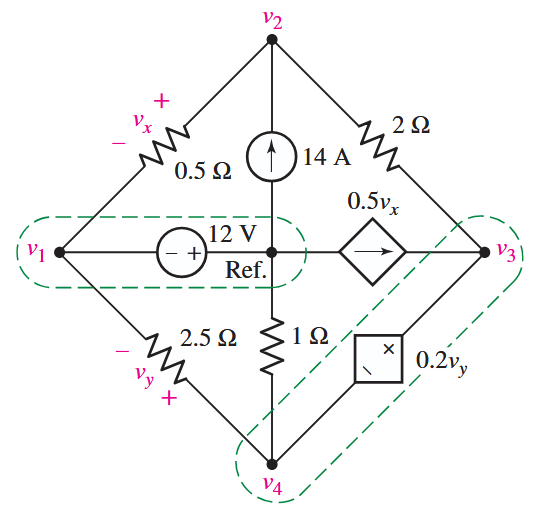
\includegraphics[width=0.5\textwidth]{Supernode.png}
\end{center}
\underline{At node 1}, we are given the voltage from the voltage source
\[v_1 = [12\,\text{V}]\]
\underline{At node 2}, we apply KCL
\[\underbrace{\frac{v_2-v_1}{[0.5\,\Omega]} + \frac{v_2-v_3}{[2\,\Omega]} }_{\text{out}}= \underbrace{[14\,\text{A}]}_{\text{in}}\]
\underline{At the 3-4 supernode}, we get two equations
\[\underbrace{\frac{v_3-v_2}{[2\,\Omega]}+\frac{v_4}{[1\,\Omega]}+\frac{v_4-v_1}{[2.5\,\Omega]}}_{\text{out}}=\underbrace{0.5v_x}_{\text{in}} \quad \text{(KCL)}\]
Relate source voltage to node voltage, keeping consistent with the given polarity of the voltage source
\[v_3-v_4 = 0.2v_y\]
Finally, we can relate $v_x$ and $v_y$ to the node voltages as well
\[v_x = v_2 - v_1\]
\[v_y = v_4 - v_1\]
\underline{Note:} Supernodes must produce two equations because they contain two unknown node voltages. When defining the voltage difference across a resistor, we subtract from the voltage at the first node encountered, since there is a voltage drop in the direction of current flow; this keeps the voltage difference positive and consistent with the assumed current directions in the KCL equation.
\section*{Mesh Analysis}
Mesh analysis is a direct application of KVL to the loops of a circuit, to use it we follow these steps:
\begin{enumerate}
    \item Identify the meshes (unique loops) in the circuit and assign a mesh current to each mesh (unknowns), note the positive direction of current.
    \item Apply KVL to each mesh, using Ohm's law to express voltages in terms of mesh currents.
\end{enumerate}  
\textbf{Supermesh}\\
When two meshes have a \textit{current source} (independent or dependent) in common, we can treat those two meshes as a single \textbf{supermesh}, going \textit{around} the current source and ignoring it. We will still get two equations from the supermesh, one from KVL and one from relating the mesh currents to the current source. For example:
\begin{center}
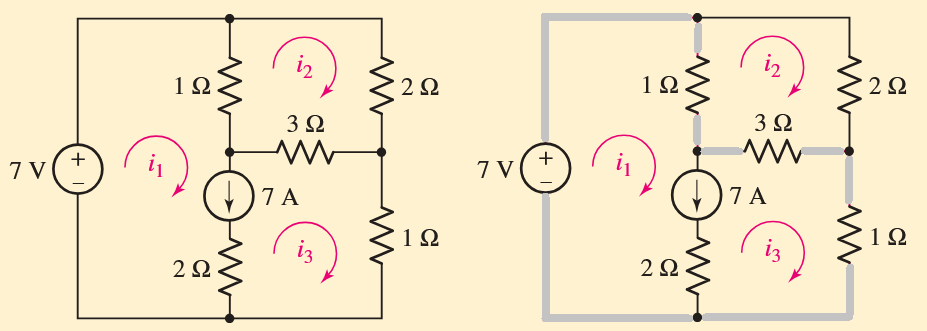
\includegraphics[width=0.7\textwidth]{Supermesh.png}
\end{center}
(Left) A three mesh circuit with a shared current source. (Right) A supermesh defined by the thick grey line.\\\\
\underline{Supermesh KVL equation}
\[[7\,\text{V}]-(i_1-i_2)[1\,\Omega]-(i_3-i_2)[3\,\Omega]-i_3[1\,\Omega]=0\]
Relating the mesh currents to the current source, keeping consistent with the \textit{given} direction of the current source
\[i_1-i_3 = [7\,\text{A}]\]
\underline{Mesh 2}
\[-(i_2-i_1)[1\,\Omega]-i_2[2\,\Omega]-(i_2-i_3)[3\,\Omega]=0\]
\underline{Note:} When moving across a voltage source, it is a voltage rise (positive voltage) if we move (-) to (+) and a voltage drop (negative voltage) if we move (+) to (-). When moving across resistors, we assume a direction of current flow and subtract the voltage drop, subtracting opposing mesh currents from the mesh current in the direction of the assumed current flow.\\\\
Both nodal and mesh analysis are \textit{always} valid and applicable since they are just applying Kirchoff's laws. However, we pick the method that results in the system of equations with the fewer unknowns.
\section*{Voltage Division in a Series Circuit}
The voltage divider rule lets us find the voltage across a series resistor without having to solve for the current first.\\
\begin{minipage}{0.6\textwidth}
\[v_1 = v \frac{R_1}{R_1 + R_2}\]
\[v_2 = v \frac{R_2}{R_1 + R_2}\]
Generalizing this rule for $N$ resistors in series, we have
\[\boxed{V_k = \frac{R_k}{R_1+R_2+\cdots+R_N} V_s}\]
\end{minipage}
\hfill
\begin{minipage}{0.3\textwidth}
    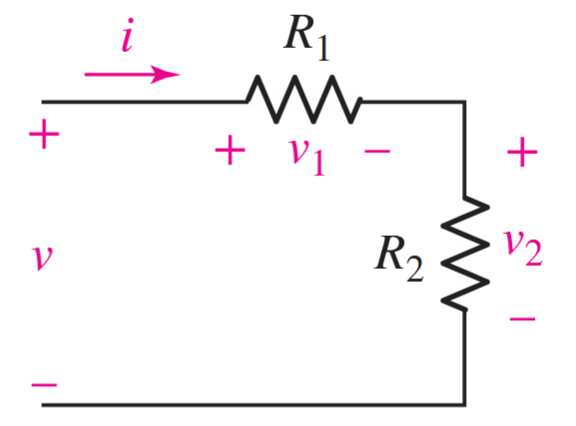
\includegraphics[width=\textwidth]{Voltage Division.png}
\end{minipage}

\section*{Current Division in a Parallel Circuit}
Current division rule lets us find the current through a parallel resistor without having to solve for the voltage first.\\
\begin{minipage}{0.6\textwidth}
\[i_1 = i \frac{R_2}{R_1 + R_2}\]
\[i_2 = i \frac{R_1}{R_1 + R_2}\]
\textbf{The currents depend on the resistor on the other branch.}\\\\
Generalizing this rule for $N$ resistors in parallel, we have
\[\boxed{I_k = \frac{\frac{1}{R_k}}{\frac{1}{R_1} + \frac{1}{R_2} + \cdots + \frac{1}{R_N}} I_s}\]
\end{minipage}
\hfill
\begin{minipage}{0.3\textwidth}
    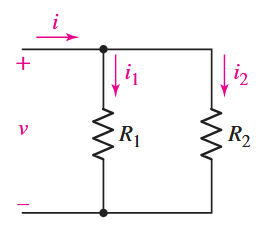
\includegraphics[width=\textwidth]{Current Division.png}
\end{minipage}
\section*{Superposition}
Since circuit elements are linear, we can analyze the contributions from \textit{independent} sources (voltage or current) separately and then add them up to get the total response. In other words, if we want to know the voltage or current across a particular element, we can find the contribution from each independent source by turning off all the other independent sources and then add up the contributions.
\begin{itemize}
    \item When turning off an independent voltage source, it becomes a \textbf{short circuit} (0 V across its terminals).
    \item When turning off an independent current source, it becomes an \textbf{open circuit} (0 A through its terminals).
\end{itemize}
If $i_x'$ and $i_x''$ are the contributions to the current $i_x$ from two independent sources, then by superposition we have
\[\boxed{i_x = i_x' + i_x''}\]
Likewise for voltage, if $v_x'$ and $v_x''$ are the contributions to the voltage $v_x$ from two independent sources, then by superposition we have
\[\boxed{v_x = v_x' + v_x''}\]
\underline{Note:} These sources need not be the same type of source, their contributions can still be added together.
\section*{Source Transformation}
Source transformation can be used to simplify and rewrite circuits. A voltage element in series with a resistor can be transformed into a current element in parallel with the same resistor, and vice versa. 
\begin{center}
    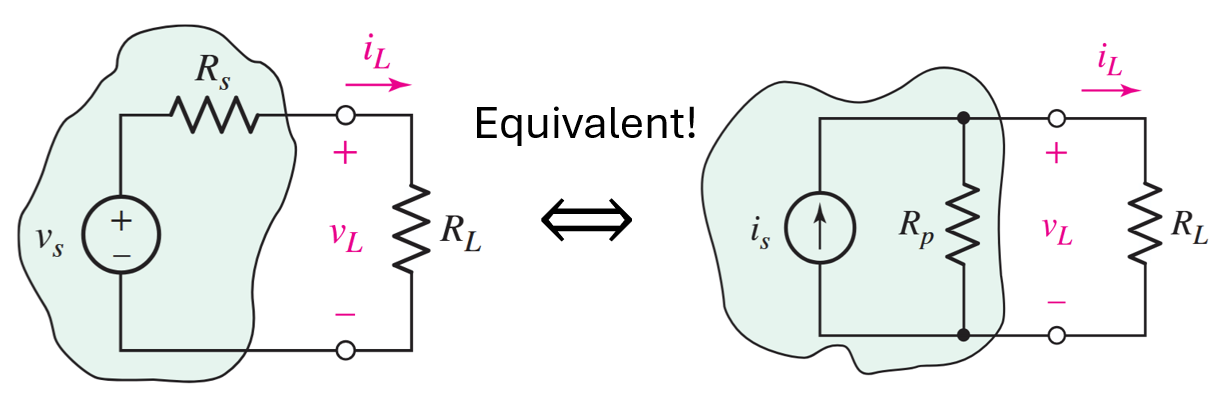
\includegraphics[width=0.8\textwidth]{Source Transformation.png}
\end{center}
These two circuits are equivalent if
\[\boxed{R_s = R_p \quad \text{AND} \quad v_s = i_sR_s}\]
The load $R_L$ connected to the terminals of $v_L$ and $i_L$ will see the same voltage and current in both circuits, thus they are equivalent.
\underline{Note:} This is also how non-ideal voltage and current sources can be modeled, where $R_s$ and $R_p$ represent the internal resistance of the source.
\section*{Delta-Wye Transformation}
Sometimes we have a circuit with a triangle (delta) of resistors that we want to convert to a Y (wye) of resistors, or vice versa. The delta-wye transformation allows us to do this.
\begin{center}
    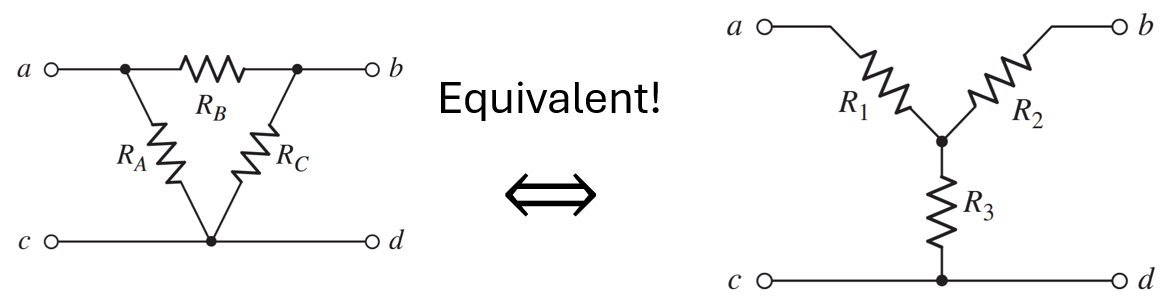
\includegraphics[width=0.8\textwidth]{Delta Wye.png}
\end{center}
\textbf{The Delta ($\Delta$) is Equivalent to the Wye ($Y$) if}
\[\boxed{
\begin{aligned}
R_A &= \frac{R_1 R_2 + R_2 R_3 + R_3 R_1}{R_2} \\
R_B &= \frac{R_1 R_2 + R_2 R_3 + R_3 R_1}{R_3} \\
R_C &= \frac{R_1 R_2 + R_2 R_3 + R_3 R_1}{R_1}
\end{aligned}}\]
\textbf{The Wye ($Y$) is Equivalent to the Delta ($\Delta$) if}
\[\boxed{\begin{aligned}
R_1 &= \frac{R_A R_B}{R_A + R_B + R_C} \\
R_2 &= \frac{R_B R_C}{R_A + R_B + R_C} \\
R_3 &= \frac{R_C R_A}{R_A + R_B + R_C}
\end{aligned}}\]
Be very careful when keeping track of what each resistor is in the delta and wye.


\end{document}